\documentclass[11pt]{article} % Font size
%%%%%%%%%%%%%%%%%%%%%%%%%%%%%%%%%%%%%%%%%
% Wenneker Assignment
% Structure Specification File
% Version 2.0 (12/1/2019)
%
% This template originates from:
% http://www.LaTeXTemplates.com
%
% Authors:
% Vel (vel@LaTeXTemplates.com)
% Frits Wenneker
%
% License:
% CC BY-NC-SA 3.0 (http://creativecommons.org/licenses/by-nc-sa/3.0/)
% 
%%%%%%%%%%%%%%%%%%%%%%%%%%%%%%%%%%%%%%%%%

%----------------------------------------------------------------------------------------
%	PACKAGES AND OTHER DOCUMENT CONFIGURATIONS
%----------------------------------------------------------------------------------------

\usepackage{amsmath, amsfonts, amsthm} % Math packages
\usepackage[stable]{footmisc}
\usepackage{listings} % Code listings, with syntax highlighting

 % English language hyphenation

\usepackage{graphicx} % Required for inserting images
\graphicspath{{Figures/}{./}} % Specifies where to look for included images (trailing slash required)

\usepackage{booktabs} % Required for better horizontal rules in tables

\numberwithin{equation}{section} % Number equations within sections (i.e. 1.1, 1.2, 2.1, 2.2 instead of 1, 2, 3, 4)
\numberwithin{figure}{section} % Number figures within sections (i.e. 1.1, 1.2, 2.1, 2.2 instead of 1, 2, 3, 4)
\numberwithin{table}{section} % Number tables within sections (i.e. 1.1, 1.2, 2.1, 2.2 instead of 1, 2, 3, 4)

\setlength\parindent{0pt} % Removes all indentation from paragraphs

\usepackage{enumitem} % Required for list customisation
\setlist{noitemsep} % No spacing between list items

\usepackage{color}

%----------------------------------------------------------------------------------------
%	DOCUMENT MARGINS
%----------------------------------------------------------------------------------------
\usepackage[utf8]{vietnam}
\usepackage[english]{babel}
\usepackage[utf8]{inputenc}
\usepackage{geometry} % Required for adjusting page dimensions and margins

\geometry{
	paper=a4paper, % Paper size, change to letterpaper for US letter size
	top=2.5cm, % Top margin
	bottom=3cm, % Bottom margin
	left=3cm, % Left margin
	right=3cm, % Right margin
	headheight=0.75cm, % Header height
	footskip=1.5cm, % Space from the bottom margin to the baseline of the footer
	headsep=0.75cm, % Space from the top margin to the baseline of the header
	%showframe, % Uncomment to show how the type block is set on the page
}

%----------------------------------------------------------------------------------------
%	FONTS
%----------------------------------------------------------------------------------------





%----------------------------------------------------------------------------------------
%	HEADERS AND FOOTERS
%----------------------------------------------------------------------------------------

\usepackage{scrlayer-scrpage} % Required for customising headers and footers

\ohead*{} % Right header
\ihead*{} % Left header
\chead*{} % Centre header

\ofoot*{} % Right footer
\ifoot*{} % Left footer
\cfoot*{\pagemark} % Centre footer
\usepackage[unicode]{hyperref}
 % Include the file specifying the document structure and custom commands
%----------------------------------------------------------------------------------------
%	TITLE SECTION
%----------------------------------------------------------------------------------------
\title{	
	\normalfont\normalsize
	\textsc{VNUHCM - University of Science \\Faculty of Information Technology}\\ % Your university, school and/or department name(s)
	\vspace{25pt} % Whitespace
	\rule{\linewidth}{0.5pt}\\ % Thin top horizontal rule
	\vspace{20pt} % Whitespace
	{\huge Lab01 - Search Problem}\\ % The assignment title
	\vspace{12pt} % Whitespace
	\rule{\linewidth}{2pt}\\ % Thick bottom horizontal rule
	\vspace{12pt} % Whitespace
}

\author{\LARGE 19120212- Vũ Công Duy \\ \LARGE 19120389 - Tô Gia Thuận}
\date{\normalsize\today} % Today's date (\today) or a custom date
\begin{document}
\maketitle 
\begin{figure}[h] % [h] forces the figure to be output where it is defined in the code (it suppresses floating)
	\centering
	
\includegraphics[width=0.4\columnwidth]{hcmus.png} % Example image
\end{figure}
\tableofcontents% tạo mục lục
%------------------------------------------------
\newpage
\section{Bảng phân công}
% Please add the following required packages to your document preamble:
% \usepackage{graphicx}
% Please add the following required packages to your document preamble:
% \usepackage{graphicx}
% Please add the following required packages to your document preamble:
% \usepackage{booktabs}
% \usepackage{graphicx}
% Please add the following required packages to your document preamble:
% \usepackage{booktabs}
% \usepackage{graphicx}
\begin{table}[h]
	\resizebox{\textwidth}{!}{%
	\begin{tabular}{@{}|l|l|l|@{}}
	\toprule
	Công việc                                            & Vũ Công Duy - 19120212 & Tô Gia Thuận - 19120389 \\ \midrule
	Thiết kế chương trình                                & x                      &                         \\ \midrule
	Viết mã nguồn phần trừu tượng                        & x                      &                         \\ \midrule
	Cài đặt thuật toán                                   & x                      &                         \\ \midrule
	Thiết kế cấu trúc bài toán mê cung                   &                        & x                       \\ \midrule
	Viết mã nguồn phần đặc biệt hóa bài toán mê cung     &                        & x                       \\ \midrule
	Thiết kế giao diện chương trình, đồ họa              &                        & x                       \\ \midrule
	Thiết kế bản đồ                                      &                        & x                       \\ \midrule
	Thiết kế cấu trúc bài toán có điểm thưởng            & x                      &                         \\ \midrule
	Viết mã nguồn phần đặc biệt hóa bài toán điểm thưởng & x                      & x                       \\ \midrule
	Kiểm thử chương trình                                & x                      & x                       \\ \midrule
	Viết báo cáo (ai làm phần nào báo cáo phần đó)       & x                      & x                       \\ \bottomrule
	\end{tabular}%
	}
	\end{table}
\section{Mô tả đồ án}
\subsection{Dẫn nhập}
Từ xa xưa, con người luôn muốn tìm cách tối ưu một công việc nào đó, điều đó cũng rất đúng khi áp dụng trong việc tìm kiếm đường đi. Làm thế nào để có thể lựa chọn đường đi ngắn nhất, ít vật cản nhất khi đi từ điểm A đến điểm B. Nhưng cũng có lúc cũng chỉ quan tâm đến cách để đi từ điểm A đến B sao cho chi phí thấp nhất mà không cần quan tâm đến độ dài đường đi. Từ đó những vấn đề thực tiễn đó, chúng ta đưa ra khải niệm về bài toán tìm đường đi trong một không gian ma trận MxN.
\subsection{Yêu cầu đồ án} \cite{slide}
 Áp dụng các thuật toán tìm kiếm không có thông tin và có thông tin để tìm đường đi thoát khỏi mê cung. 
\\- Kí hiệu \textbf{Ngôi sao} trong mê cung đánh dấu điểm bắt đầu của vật thể. 
\\- Kí hiệu \textbf{X} biểu diễn các bức tường chắn của mê cung.
\\- Kí hiệu \textbf{EXIT} đánh dấu lối thoát của mê cung
\\Yêu cầu đồ án: Áp dụng 4 thuật toán DFS, BFS, GBFS, A* để tìm đường đi thoát khỏi mê cung đồng thời đi qua các các điểm thưởng.
\begin{figure}[h] % [h] forces the figure to be output where it is defined in the code (it suppresses floating)
	\centering
	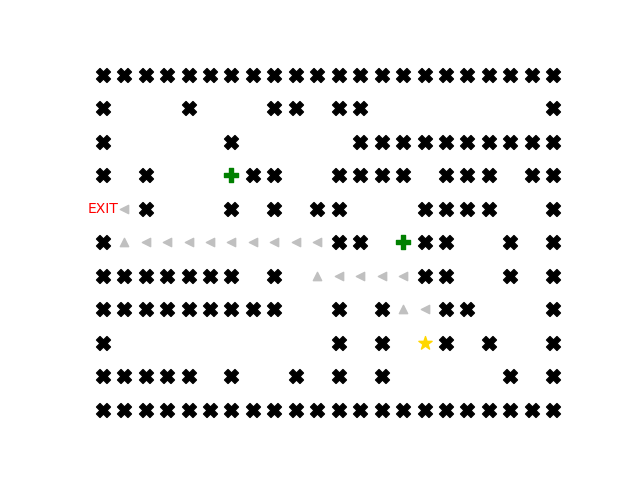
\includegraphics[width=0.5\columnwidth]{demo_maze.png} % Example image
\end{figure}
\section{Hướng dẫn sử dụng chương trình}

Chương trình khi khởi động sẽ có 2 lựa chọn, người dùng nhập vào 1 hoặc 2 tương ứng với :\\
- 1.Chạy thuật toán tìm đường đi với \textbf{bản đồ không điểm thưởng} và trực quan hóa cách giải(bao gồm đường đi và các điểm đã khám phá). Chạy hết 5 bản đồ được đánh số từ 1-5.\\
- 2.Chạy thuật toán tìm đường đi với \textbf{bản đồ có điểm thưởng} và trực quan hóa đường đi. Chạy hết 5 bản đồ được đánh số từ 6-8.\\
Chi tiết :\\
1. Chạy chương trình: chạy file \textbf{main.py} chứa chương trình chính
\begin{figure}[h] 
	\centering
	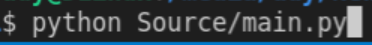
\includegraphics[width=0.5\columnwidth]{Figures/hdsd_1.png}
\end{figure}\\
2. Lựa chọn phần muốn chạy được nêu chi tiết ở phần trên.
\begin{figure}[h] 
	\centering
	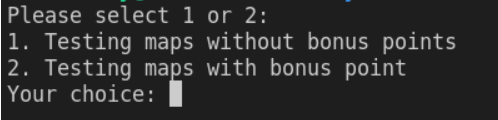
\includegraphics[width=0.5\columnwidth]{Figures/hdsd_3.png}
\end{figure}\\
3. Với mỗi map, chương trình sẽ hiển thị : quá trình mở rộng trạng thái, các bước thực hiện đường đi kết quả, tổng số điểm đã mở rộng, chi phí đường đi kết quả và trực quan hóa những điều đó lên trên một cửa sổ đồ họa. \\ Người dùng muốn lưu lại có thể ấn nút lưu trên bản đồ.\\
\begin{figure}[h] 
	\centering
	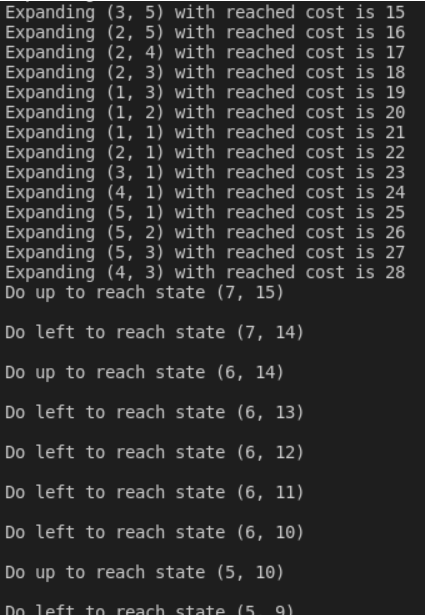
\includegraphics[width=0.5\columnwidth]{Figures/hdsd_4.png}
\end{figure}\\

\begin{figure}[h] 
	\centering
	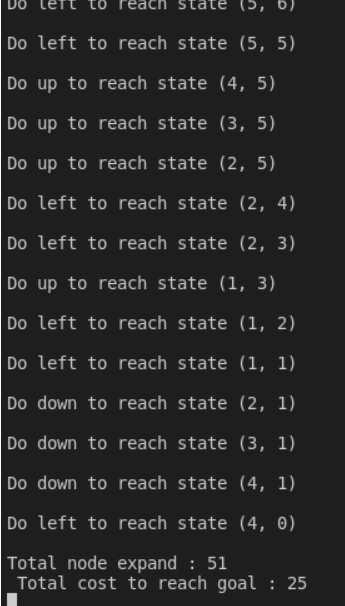
\includegraphics[width=0.5\columnwidth]{Figures/hdsd_5.png}
\end{figure}

4. Ấn dấu x trên bản đồ để chương trình chạy map hoặc thuật toán tiếp theo đến khi không còn gì để chạy.\\
\newpage
\begin{figure}[h] 
	\centering
	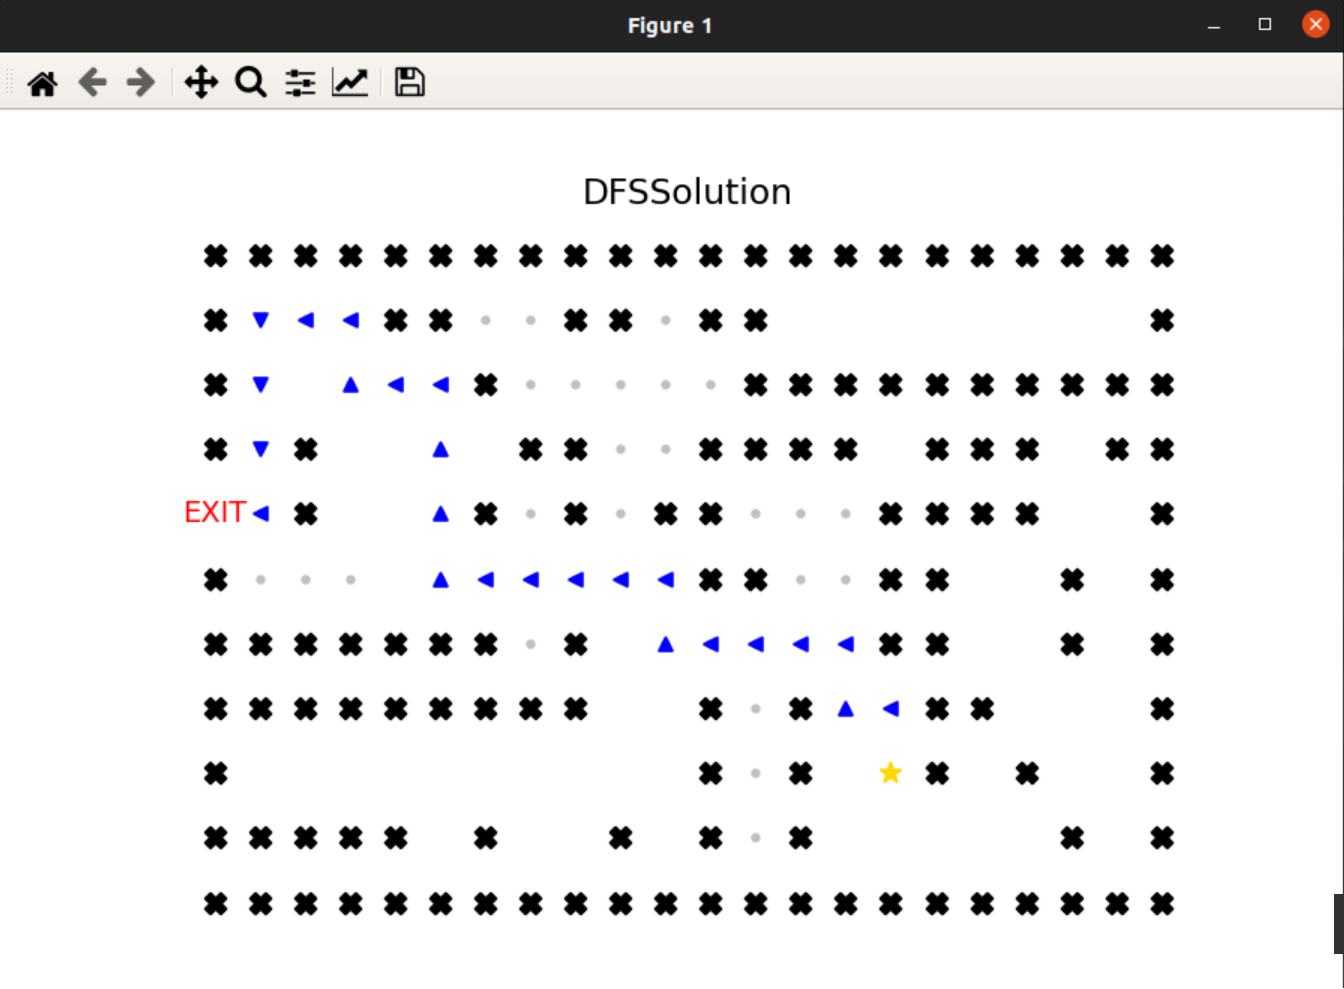
\includegraphics[width=0.5\columnwidth]{Figures/hssd_2.png}
\end{figure}
\section{Xây dựng cấu trúc chương trình} 
\footnote{Ý tưởng trừu tượng hóa vấn đề được tham khảo ở khóa CS221 của đại học Stanford \cite{standfordcs221}}
Mục tiêu của việc xây dựng cấu trúc chương trình là để việc cài đặt những thuật toán được tổng quát hóa, giúp cài đặt những bài toán khác nhau và giải chúng bằng nhiều thuật toán khác nhau trở nên đơn giản hơn. 

Theo cách nói của những nhà phát triển phần mềm, mã nguồn có thể được tái sử dụng trong nhiều trường hợp khác nhau, giúp người lập trình có thể tập trung hơn vào phần tối ưu thuật toán mà không nghĩ ngợi nhiều về phần kỹ thuật, cài đặt.

Việc cài đặt dựa chủ yếu vào kỹ thuật kế thừa, đa hình trong kỹ thuật lập trình hướng đối tượng. Chương trình sẽ được trực quan hóa bằng biểu đồ UML sau đây.

\newpage
\begin{figure}[h] % [h] forces the figure to be output where it is defined in the code (it suppresses floating)
	\centering
	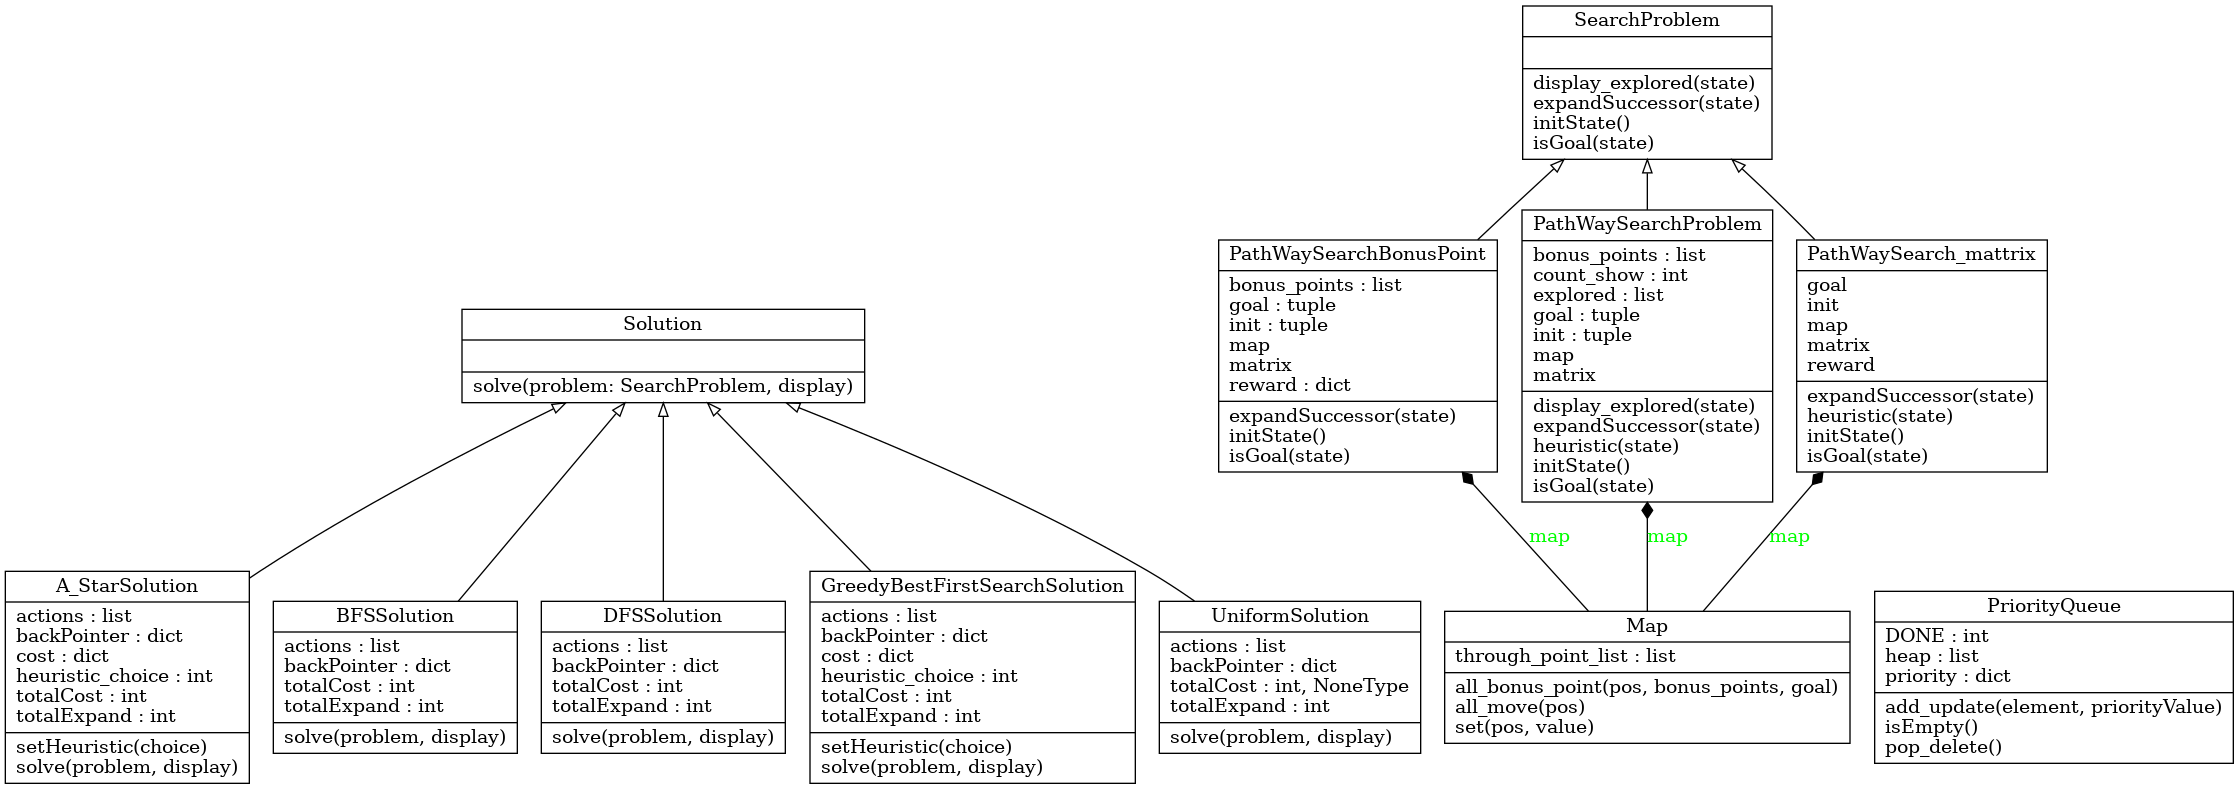
\includegraphics[width=1.2\columnwidth]{Figures/UML.png} % Example image
\end{figure}

\subsection{Hai class trừu tượng (Abstract Class)}
Ở level cao nhất chính là 2 class : Solutimethodon và SearchProblem tương ứng với hai thực thể (entity) là lời giải và bài toán.

Ở abstract class, phương thức (method) sẽ được cài đặt dưới dạng phương thức ảo (virtual method), những phương thức này sẽ được các lớp con kế thừa và được cài đặt trong quá trình viết các lớp con ấy.

Để tránh trường hợp method của abstract class được gọi (có thể do method của class kế thừa chưa được cài đặt), ta sẽ thêm dòng báo lỗi khi method của abstract class được gọi raise NotImplementedError(...)

%------------------------------------------------
\lstinputlisting[
	caption=Cài đặt abstract class, % Caption above the listing
	label=lst:luftballons, % Label for referencing this listing
	language=Perl, % Use Perl functions/syntax highlighting
	frame=single, % Frame around the code listing
	showstringspaces=false, % Don't put marks in string spaces
	numbers=left, % Line numbers on left
	numberstyle=\tiny, % Line numbers styling
	]{abstract_class.txt}

Cấu trúc của bài toán cũng như những "nguyên liệu" để giải bài toán ấy như : trạng thái ban đầu(init state), trạng thái đích(goals), mở rộng trạng thái kề(expand successor)\cite{csttnt_lhb},... được biểu diễn dưới dạng các phương thức của một thực thể của class SearchProblem. 

Ở class Solution, phương thức duy nhất là solve(problem,display) sẽ được truyền vào tham số là một thực thể của class SearchProblem. Phương thức solve sẽ được cài đặt một cách trừu tượng để có thể giải được bất cứ bài toán tìm kiếm nào dựa vào những "nguyên liệu" được lấy từ thực thể class SearchProblem truyền vào.

Phương thức display\_explored(state) của class SearchProblem có nhiệm vụ trực quan hóa trạng thái hiện tại để quá trình cài đặt thuật toán thuận lợi hơn, không bắt buộc có. Vì vậy, class kế thừa SeachProblem không bắt buộc cài đặt phương thức này, ta cho lệnh "pass" (bỏ qua) nếu phương thức này được gọi từ abstract class.

\subsection{Class PriorityQueue}
Đây là lớp hàng đợi ưu tiên được bổ sung một vài tính năng để tối ưu cho bài toán tìm kiếm.

Các tính năng bổ sung bao gồm : không push lại những phần tử đã được pop, update chỉ số ưu tiên nếu chỉ số ưu tiên mới lớn hơn chỉ số cũ. 
\lstinputlisting[
	caption=Cài đặt class PriorityQueue, % Caption above the listing
	label=lst:luftballons, % Label for referencing this listing
	language=Perl, % Use Perl functions/syntax highlighting
	frame=single, % Frame around the code listing
	showstringspaces=false, % Don't put marks in string spaces
	numbers=left, % Line numbers on left
	numberstyle=\tiny, % Line numbers styling
]{priority_queue.txt}

Thuộc tính \textbf{heap} là một list các tuple (element, value).Việc sắp xếp, pop, push các phần tử theo cấu trúc heap được thực hiện bởi hàm heappush trong thư viện heapq của python3.

Thuộc tính \textbf{priority} là một dict lưu trữ các element đã được thêm vào heap (kể cả các element đã được pop khỏi heap) và value của mỗi element đó. Những element nào đã được pop ra sẽ được gán value bằng với thuộc tính \textbf{DONE} mang giá trị $- \infty$ để phân biệt với các giá trị khác, thuận tiện cho việc viết điều kiện rẽ nhánh cho chương trình bỏ qua update hoặc thêm vào heap nếu đã được pop.
\subsection{Các class kế thừa Solution}
Phần này sẽ giải thích các class kế thừa abstract tức những thuật toán cụ thể
\subsubsection{BreadFirstSearch}
Đầu tiên ta khởi tạo những biến sau đây:  

- totalCost : lưu trữ tổng chi phí đường đi  

- toltaExpand : lưu trữ tổng số node mở rộng  

- action : dãy các action thực hiện để biến initState thành goalState  

- backPointer : là hashtable với key là trạng thái và value là các cặp (state,backPointer) với backPointer là trạng thái phía trước.  

- frontier : là một hàng đợi. Sẽ lưu các cặp (state,cost) sẽ được visit.  

Ta sẽ khởi tạo frontier chứa initState. Các biến khác khởi tạo bằng 0 hoặc rỗng.  

Quy trình thực hiện thuật toán được thực hiện như sau:
- Dequeue frontier, sẽ được một cặp state và chi phí để đi đến state đó.

- Tăng totalExpand lên 1 đơn vị.  

- Kiểm tra trạng thái vừa pop ra có phải là trạng thái đích chưa. Nếu đúng thì dựa vào backPointer và cost để hoàn thành list action và thoát khỏi hàm.  

- Nếu chạy hàm expand() để lấy những successor và chi phí cần thêm để đi tới chúng. Nếu successor đó có trong backPointer thì bỏ qua.

- enqueue những trạng thái mới và cost của chúng.

- Cập nhật backPointer của từng trạng thái mới chính là trạng thái vừa pop ở trên.

- Lặp đến khi nào frontier hết phân tử.

\subsubsection{DepthFirstSearch}

Thực hiện giống BFS nhưng code{frontier} là một stack thay vì queue. Hàm dequeue và enequeue thay thế bằng hàm pop và push.

\subsubsection{A*}
Khởi tạo thêm hashtable cost với key là trạng thái, value là chi phí để đi đến trạng thái đó từ trạng thái ban đầu.

Thực hiện giống BFS nhưng code{frontier} là một priorityqueue(class đã được giải thích ở trên) thay vì queue. Hàm dequeue và enequeue thay thế bằng hàm add\_update và pop\_delete.

Phần addupdate element : thay vì add (state,cost), ta add (state,cost + h(x)).

Thay vì dựa vào backPointer để loại successor, ta dựa vào hashtable cost.

Ngoài ra, khi add\_update element thành công thì mới bổ sung hastable cost và backPointer.



\subsubsection{BestFirstSearch}
Thực hiện giống A*.

Phần add\_update element : thay vì add (state,cost + h(x)), ta add (state,h(x)).
\subsection{Phân tích cấu trúc bài toán}
Xét mê cung trong bài toán nằm trên một hệ trục tọa độ hai chiều Oxy. Gọi \textbf{x} và \textbf{y} lần lượt là hoành độ và tung độ của tác nhân.\\
- Trạng thái của tác nhân: Tọa độ (x,y) trên ma trận.\\
- Trạng thái bắt đầu (start state): Tọa đô ($x^{'}$,$y^{'}$) của kí hiệu \textbf{Ngôi sao} trên ma trận.\\
- Trạng thái kết thúc (goal state): Tọa độ ($x^{''}$,$y^{''}$) của kí hiệu \textbf{EXIT} trên ma trận.\\
- Hành động của tác nhân: Di chuyển lên trên, xuống dưới, qua trái, qua phải.\\
- Hàm kế nhiệm, kế thừa (successor function): ExpandSuccessor - dùng để lựa chọn ô kế nhiệm ô cũ và cập nhật lại vị trí hiện tại của tác nhân.\\
- Hàm kiểm tra kết thúc: isGoal - kiểm tra trạng thái tác nhân đang xét (x,y) có phải là ô kết thúc (lối ra của mê cung) hay không.
\subsection{Chi tiết cách phát sinh ô kế nhiệm và chi phí}
Để cái đặt các thuật toán tìm kiếm trên ma trận có kích thước MxN, ta cần xây dựng một danh sách các điểm kề với điểm tại vị trí đang xét và chi phí phát sinh giữa điểm đang xét và các cạnh kề của nó.\\

Gọi ô (vị trí) của tác nhân tại một điểm nhất định là (x,y) trong ma trận, ứng với các hướng di chuyển lên, xuống, trái, phải, ta sẽ có các ô kề với tọa độ lần lượt là (x,y-1), (x,y+1), (x-1,y), (x+1,y). Do các ô có kích thước là như nhau nên chi phí di chuyển tới các ô kề sẽ là như nhau và trong đồ án này sẽ được đặt mặc định là 1.\\
Tuy nhiên chi phi không phải lúc nào cũng là 1. Nó có thể thay đổi trong trường hợp bài toán có điểm thưởng mà sẽ được nói chi tiết ở phần tiếp theo\\
Bằng cách phát sinh các ô kề của ô mà tác nhân đang đứng, ta sẽ có thể xây dựng danh sách các ô kề và chi phí. Khi cần lấy danh sách các ô kề và chi phí của ô hiện tại mà tác nhân đang đứng (x,y), ta phát sinh ra tọa độ ô kề thứ i của u bằng công thức (x+$dx_{i}$, y+$dy_{i}$) và chi phí tương ứng là $w_{i}$ , $\forall{i\ge0}\cup{i\le4}$\\

Sau khi khởi tạo được danh sách các ô kề của ô mà tác nhân đang đứng, ta sẽ cài đặt hàm kế nhiệm để tính toán xem các ô kề có phải là bức tường chắn hay không đồng thời tính toán chi phí, và dựa trên kết quả đó để trả về những ô phù hợp có thể kế nhiệm ô hiện tại.
\section{Cơ sở lý thuyết của tính tối ưu và đầy đủ}
\footnote{\cite{csttnt_lhb}:Chương 1: mục III.4} 
Tính đầy đủ: Một thuật toán có tính đầy đủ là một thuật toán đảm bảo tìm được lời giải cuối cùng cho bài toán đưa ra.\\
Tính tối ưu: Một thuật có tính tối ưu thì có tính đầy đủ và cho ra chuỗi các hành động có chi phí thấp nhất để đạt được mục đích bài toán\\
\subsection{Tính đầy đủ}
Tất cả các thuật toán BFS,BestFirstSearch, A*, DFS đều là các thuật toán đầy đủ \textbf{trong bài toán mê cung} dựa trên cơ sở sau:\\
	Tất cả các thuật toán trên chỉ \textbf{dừng lại}(hay nói cách khác là ngừng tạo ra trạng thái mới) khi tập \textbf{frontier}(những trạng thái sẽ được khám phá) \textbf{rỗng}, điều này chỉ xảy ra khi \textbf{hàm sinh trạng thái} trả về \textbf{rỗng}, tức không có trạng thái nào được sinh ra từ không gian trạng thái nữa hay nói cách khác là \textbf{tất cả những trường hợp} đã được \textbf{vét cạn}. Nếu tồn tại \textbf{trạng thái đích} thì nó chắc chắn sẽ được \textbf{đẩy vào trong frontier} và được \textbf{khám phá}. Như vậy ta kết luận tất cả các phương pháp tìm kiếm trên đều có tính đầy đủ.\\
Tuy nhiên, với trường hợp của DFS và Best First Search, trong trường hợp không gian trạng thái là vô hạn (tức không thể vét cạn) thì sẽ mất đi tính đầy đủ bởi nếu đi sai đường, thuật toán sẽ tiếp tục đi mà không thể quay về (chỉ quay về khi không đi được nữa, mà không gian trạng thái là vô hạn).\\
Còn với BFS,A*, nếu tồn tại đích thì đích đó sẽ phải nằm ở tầng thứ n (theo chiều rộng). Thuật toán khi mở rộng đến tầng thứ n (nếu hàm heuristic của A* là tối ưu) chắc chắn sẽ tìm được trạng thái đích.\\
\subsection{Tính tối ưu}
\subsection{BFS và UCS}
Về tổng quan, BFS chỉ mở rộng theo chiều rộng của những trạng thái đã được khám phá cho đến khi tìm được trạng thái đích. Đường đi trả về sẽ là dãy các trạng thái được sinh ra và trạng thái cha, bắt đầu từ trạng thái đích và kết thúc ở trạng thái đầu.\\
Tuy nhiên trong trường hợp cụ thể là bài toán mê cung, chi phí để đi từ trạng thái này sang trạng thái khác là \textbf{bằng nhau}.\\
Lúc này, trạng thái được khám phá sẽ luôn là trạng thái có chi phí mở rộng \textbf{ít nhất}, thuật toán lại hoạt động như thuật giải.\textbf{UCS}.\\
Vì vậy, trong trường hợp \textbf{bài toán mê cung} thì \textbf{BFS} có tính \textbf{tối ưu}, còn \textbf{tổng quan} thì \textbf{không}.
\subsection{DFS,BestFirstSearch}
BestFirstSearch và DFS đều không tối ưu.\\
\textbf{BestFirstSearch} : chỉ quan tâm tới tối ưu cho bước tiếp theo chứ không quan tâm đến toán cục.\\
Ví dụ : Cho 3 điểm A,B,C, ta muốn đi A đến C, hàm heuritic cho ra $A->C = 5, A->B = 3, B->C = 3$. BestFirstSearch sẽ chọn con đường đi tiếp theo với chi phí thấp nhất là $A->B->C$ vì thuật toán luôn chọn đường đi tối ưu cho bước tiếp theo mà không quan tâm đến tối ưu toàn cục.
\textbf{DFS} : nếu đi vào một con đường \textbf{không tối ưu} nhưng vẫn \textbf{tìm ra đích} thì thuật toán vẫn sẽ trả về con đường ấy chứ không quay lại để tìm con đường tối ưu thật sự. Thứ tự chọn trạng thái con để mở rộng theo chiều sâu cũng phụ thuộc vào lúc cài đặt nên càng không tối ưu.\\
\subsection{A*}
\footnote{\cite{csttnt_lhb}, Chương 2: Mục I.2: Tìm kiếm A*} "Để đảm bảo A* tìm được lời giải tối ưu thì hàm $h(n)$ phải là hàm heuristic chấp nhận được. Hàm heuristic chấp nhận được khi nó không bao giờ ước lượng quá chi phí để đến đích thật sự."\\
Ở bài toán này, ta chọn hàm heuristic chính là khoảng cách mahatan từ nguồn đến đích. Đây là hàm heuristic chấp nhận được vì khoảng cách mahatan chính là chi phí ngắn nhất có thể nếu múôn đi từ nguồn đến đích, nên chắc chắn nó ngắn hơn đường đi thực tế với nhiều vật cản.\\
\newpage
\subsection{}
\section{Đánh giá thực nghiệm}
\subsection{Giao diện kết quả}
	\begin{figure}[h] % [h] forces the figure to be output where it is defined in the code (it suppresses floating)
		\centering
		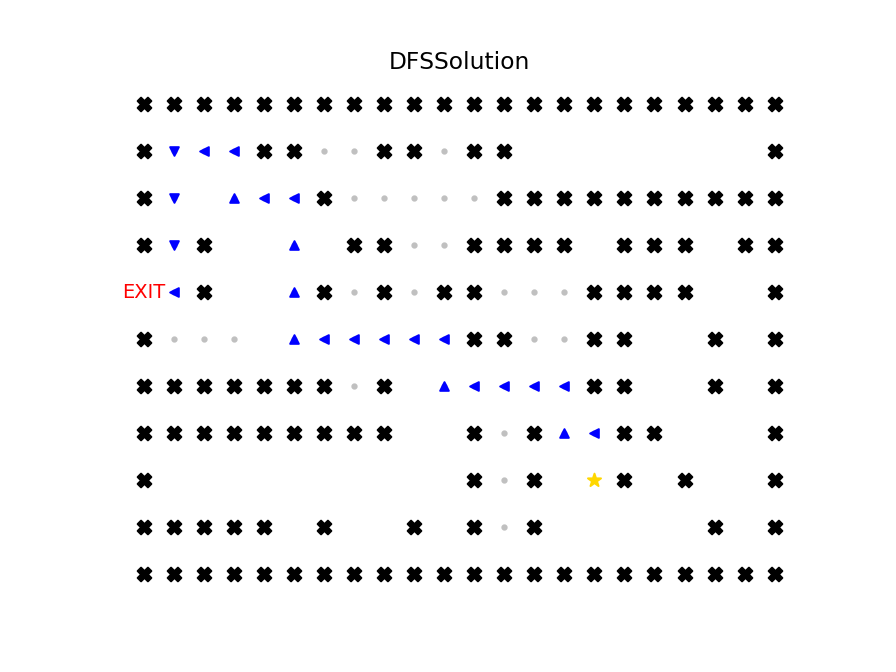
\includegraphics[width=0.8\columnwidth]{Figures/fg1_dfs.png} % Example image
	\end{figure}
\begin{itemize}
	\item DFSSolution: Tên thuật toán sử dụng (bao gồm DFSSolution, BFSSolution, GreedyBestFirstSearchSolution, A\_StarSolution) \\
	\item \textbf{$\triangle$}: Đường đi của tác nhân thoát khỏi mê cung. \\
	\item \textbf{$\bigcirc$}: Các ô đã duyệt qua (bao gồm cả ô được chọn làm đường đi và ô không được chọn làm đường đi).\\
	\item \textcolor{yellow}{\textbf{$\star$}}: Đánh dấu điểm bắt đầu của tác nhân. \\
	\item \textbf{X}: biểu diễn các bức tường chắn của mê cung.\\
	\item \textcolor{red}{EXIT} đánh dấu lối thoát của mê cung.\
\end{itemize}

\newpage
\subsection{Bản đồ không có điểm thưởng}
\begin{itemize}
	\item Bản đồ 1:
		\begin{figure}[h] \label{123}
			\centering
			\begin{tabular}{cc}
				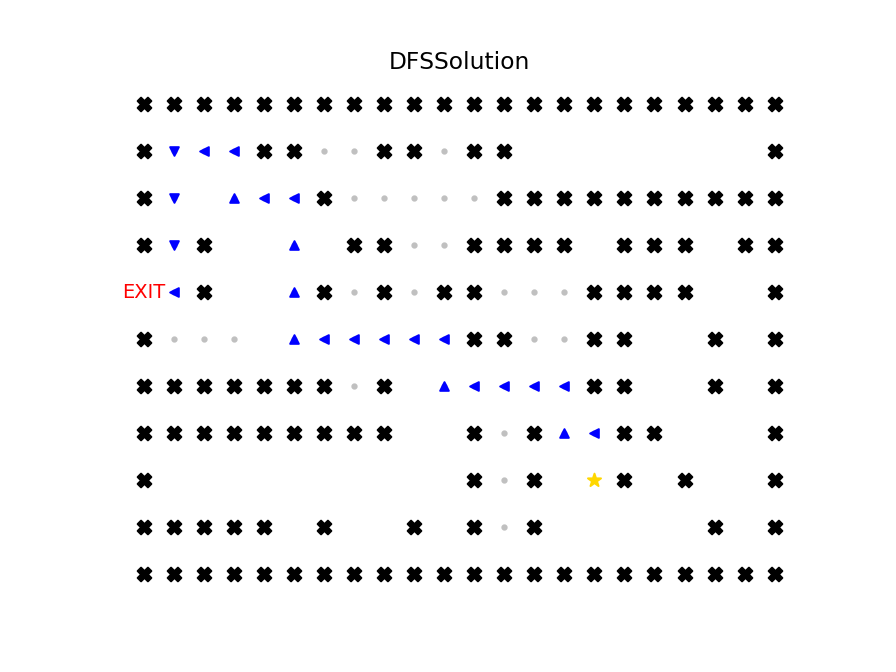
\includegraphics[width=8cm]{Figures/fg1_dfs.png} &
				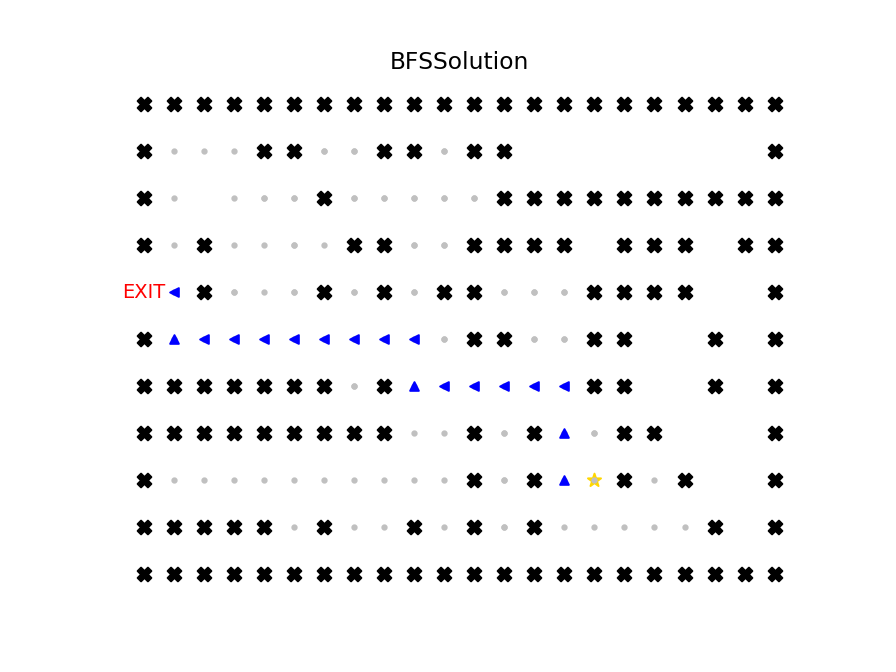
\includegraphics[width=8cm]{Figures/fg1_bfs.png} \\
			\end{tabular}
		\end{figure}
		\begin{figure}[h] \label{fig:three-alternative-operations}
			\centering
			\begin{tabular}{cc}
				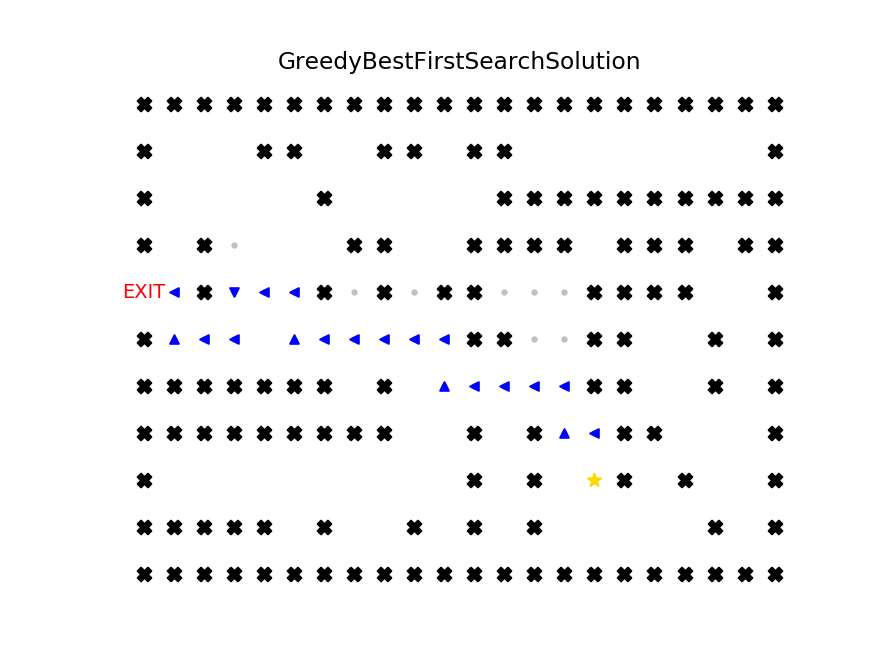
\includegraphics[width=8cm]{Figures/fg1_gbfs.png} &
				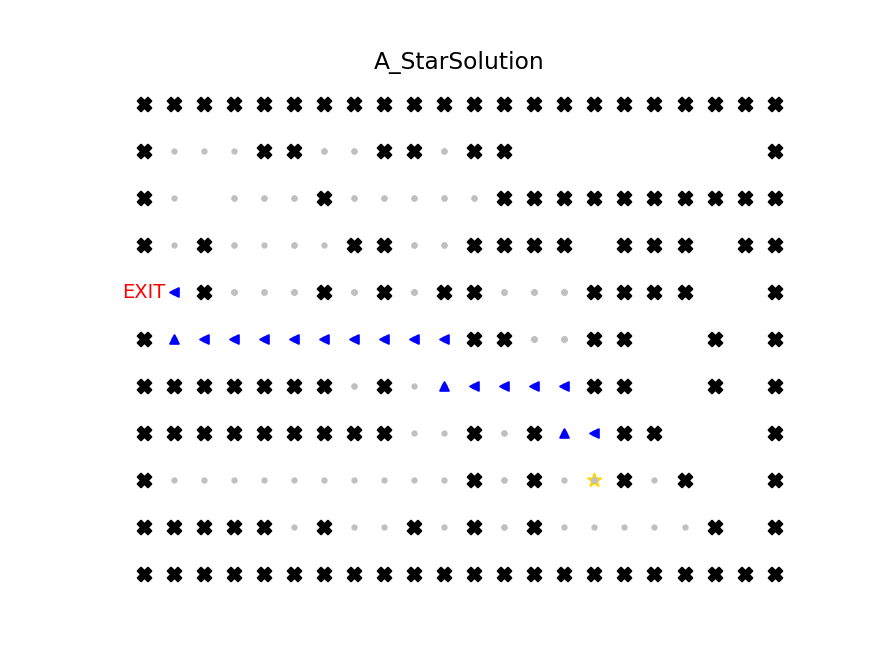
\includegraphics[width=8cm]{Figures/fg1_astar.png}
			\end{tabular}
		\end{figure}
		\begin{itemize}
			\item \textbf{Nhận xét}: Thuật toán DFS duyệt qua các điểm rất ít mà vẫn có thể tìm được đường để thoát ra khỏi mê cung, tuy nhiên đường đi tìm được không tối ưu (tìm được đường đi dài nhất trong 4 thuật toán).\\ Cả 3 thuật toán BFS, Greedy Best First Search, $A^{\star}$ cho kết quả khá tương đồng. \\Tuy nhiên Thuật toán BFS phải duyệt qua nhiều ô hơn 2 thuật toán còn lại. Đó là vì thuật toán BFS duyệt theo chiều rộng (hay còn gọi là vét cạn) nên phải duyệt qua hết tất cả mọi ô có khả năng đi qua. Như trong bản đồ này có những ô nằm trong ngõ cụt (không cần thiết phải đi qua) nhưng thuật toán BFS vẫn phải duyệt qua gây tốn chi phí về bộ nhớ và thời gian xử lí.\\Thuật toán BreadFirstSearch cho ra đường đi không tối ưu khi nó chỉ xem xét khoảng cách từ vị trí hiện tại đến đích theo đường chim bay, trong khi thực tế có vật cản là một bức tường chắn ngang nên thay vì né ra từ đầu thì thuật toán đụng tường rồi mới né, dẫn đến mất thêm chi phí.
		\end{itemize}
	
	\newpage
	\item Bản đồ 2:
	\begin{figure}[h] \label{bd2}
		\centering
		\begin{tabular}{cc}
			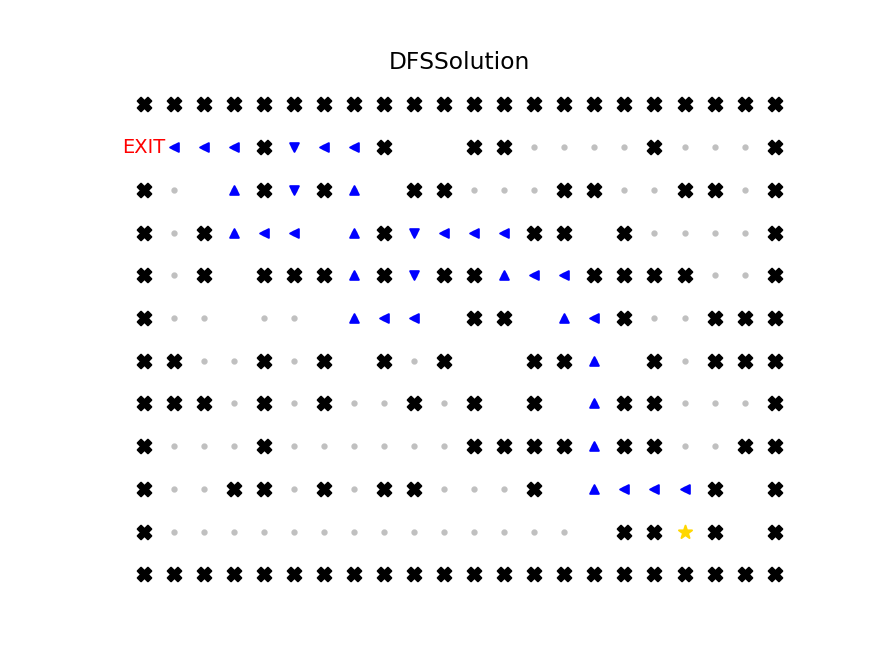
\includegraphics[width=8cm]{Figures/fg2_dfs.png} &
			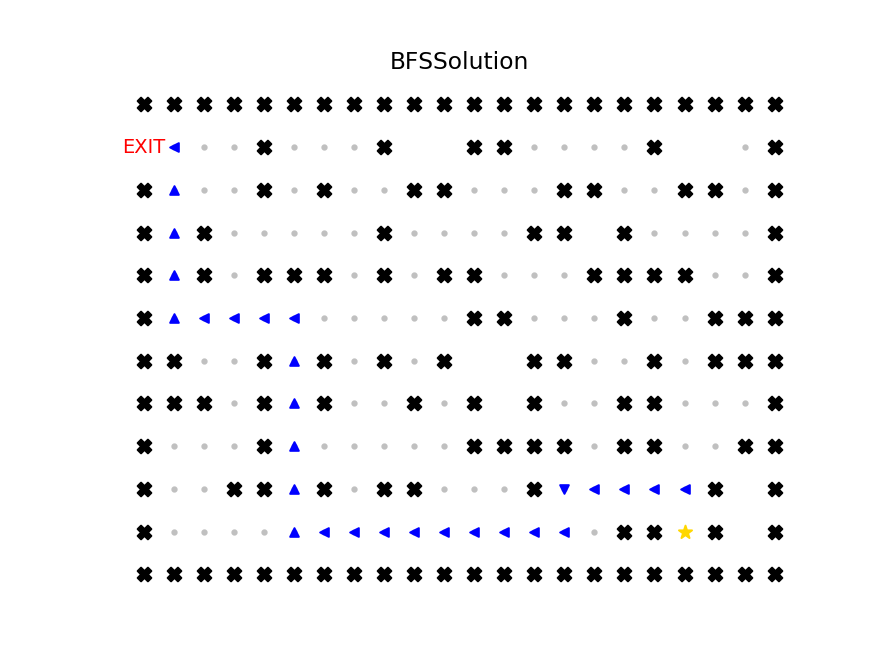
\includegraphics[width=8cm]{Figures/fg2_bfs.png} \\
		\end{tabular}
	\end{figure}
	\begin{figure}[h] \label{Hình 2}
		\centering
		\begin{tabular}{cc}
			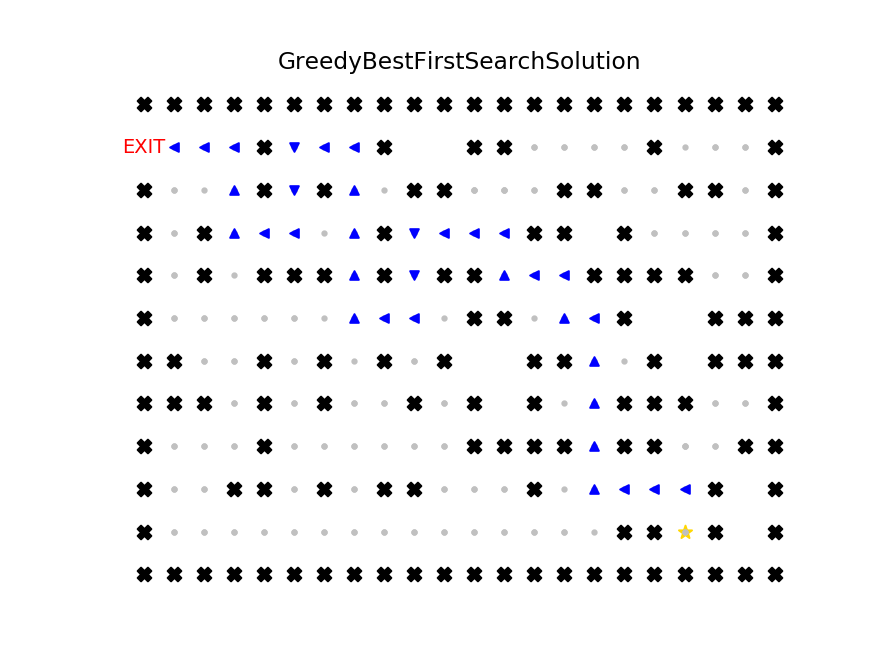
\includegraphics[width=8cm]{Figures/fg2_gbfs.png} &
			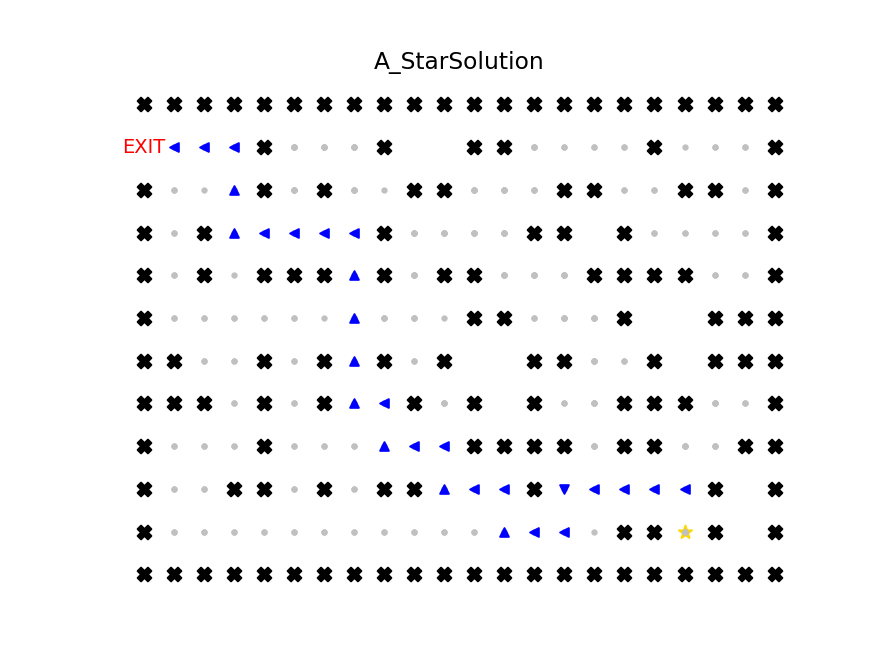
\includegraphics[width=8cm]{Figures/fg2_astar.png}
		\end{tabular}
	\end{figure}
	\begin{itemize}
		\item \textbf{Nhận xét}: Trong bản đồ này, ta dễ dàng nhận thấy thuật toán DFS và BFS hầu như duyệt qua mọi ô có thể đi, nhưng thuật toán DFS lại tìm được đường đi dài hơn. Ba thuật toán BFS, Greedy Best First Search, $A^{\star}$ tìm được những đường đi khác nhau nhưng thuật toán BFS và $A^{\star}$ lại ra đường đi có chi phí bằng nhau và ngắn nhất. Thuật toán Greedy Best First Search lại cho ra kết quả độ dài đường đi tương đương với DFS, bởi vì thuật toán GBFS sử dụng hàm heuristic để đánh giá và ước lượng để chọn đường đi, tuy nhiên do có những vật cản nên hàm heuristic đôi khi sẽ bị đánh lừa. Theo lý thuyết một ô rất gần lối thoát (dựa trên khoảng cách Manhattan) nhưng thực tế do có vật cản làm nên khi chọn ô đó để đi qua thì đường đi trở nên dài hơn và không còn được tối ưu nữa. Thuật toán $A^{\star}$ về lý thuyết cũng sử dụng hàm heuristic (khoảng cách Manhattan) nhưng đây là thuật toán dựa trên sự kết hợp từ thuật toán Dijkstra nên sẽ tính toán để tối ưu chi phí hơn, từ đó vừa tìm được đường đi ngắn vừa tối ưu được chi phí kể cả khi có vật cản.
	\end{itemize}

	\newpage
	\item Bản đồ 3:
	\begin{figure}[h] \label{bd3}
		\centering
		\begin{tabular}{cc}
			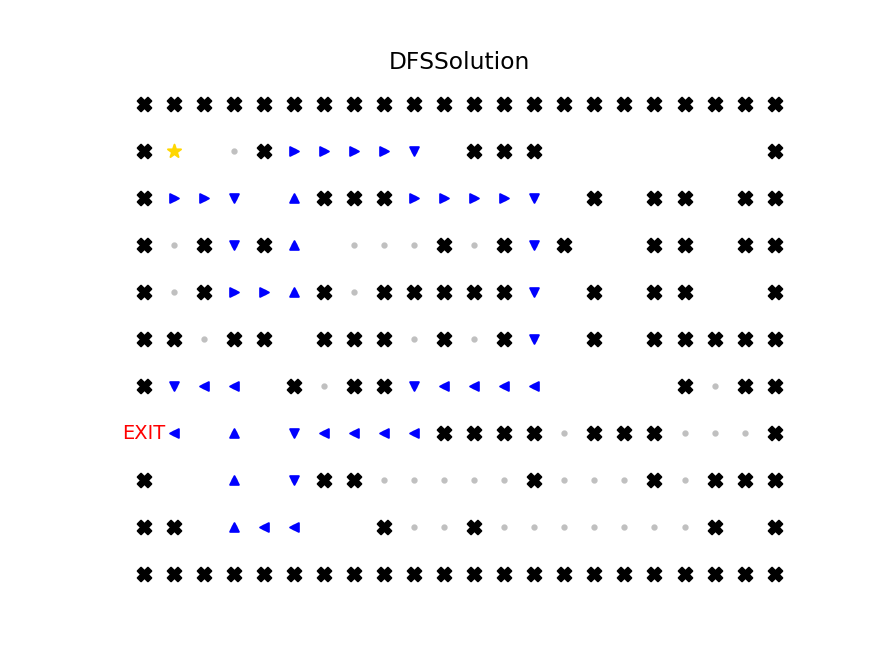
\includegraphics[width=8cm]{Figures/fg3_dfs.png} &
			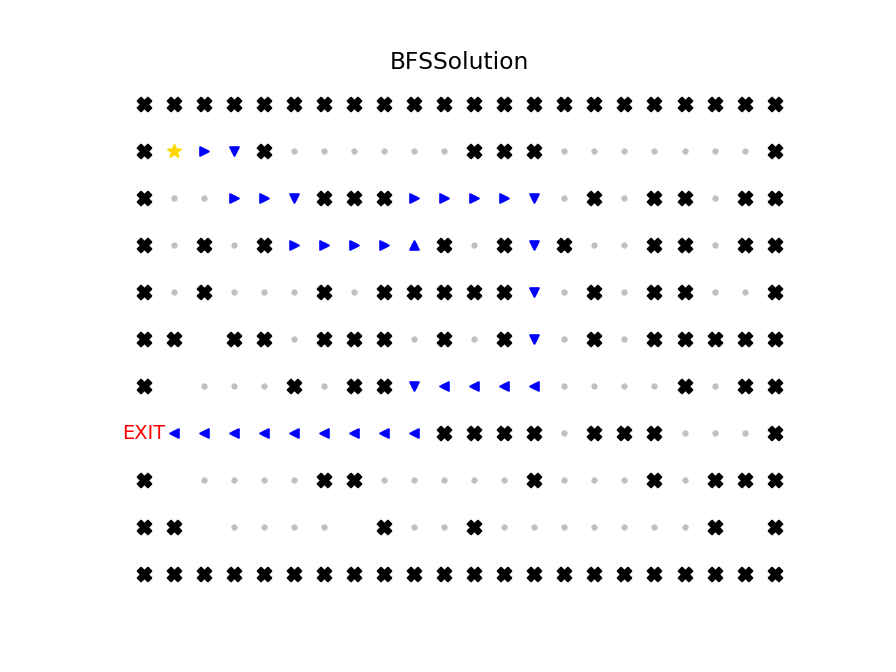
\includegraphics[width=8cm]{Figures/fg3_bfs.png} \\
		\end{tabular}
	\end{figure}
	\begin{figure}[h] \label{Hình 3}
		\centering
		\begin{tabular}{cc}
			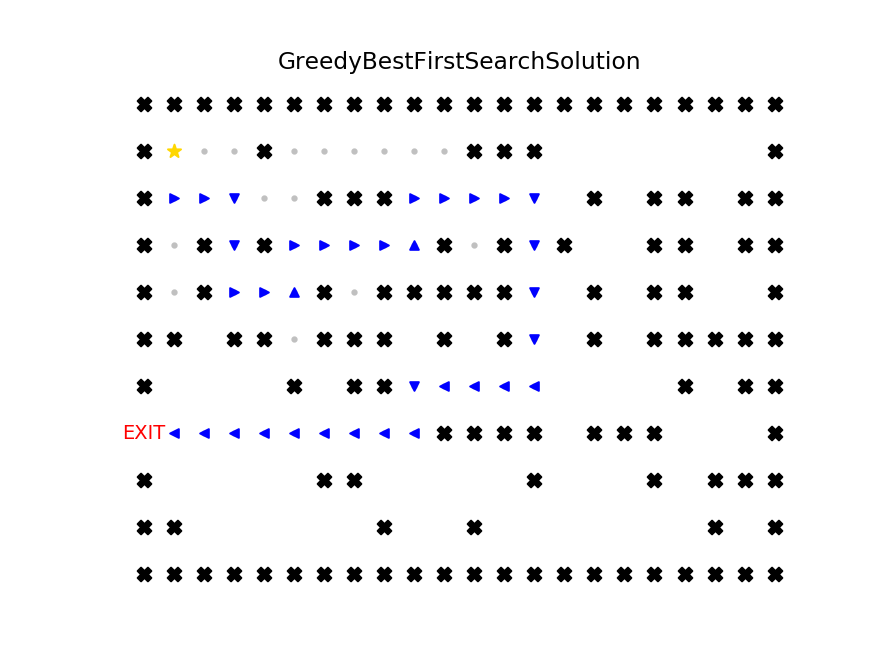
\includegraphics[width=8cm]{Figures/fg3_gbfs.png} &
			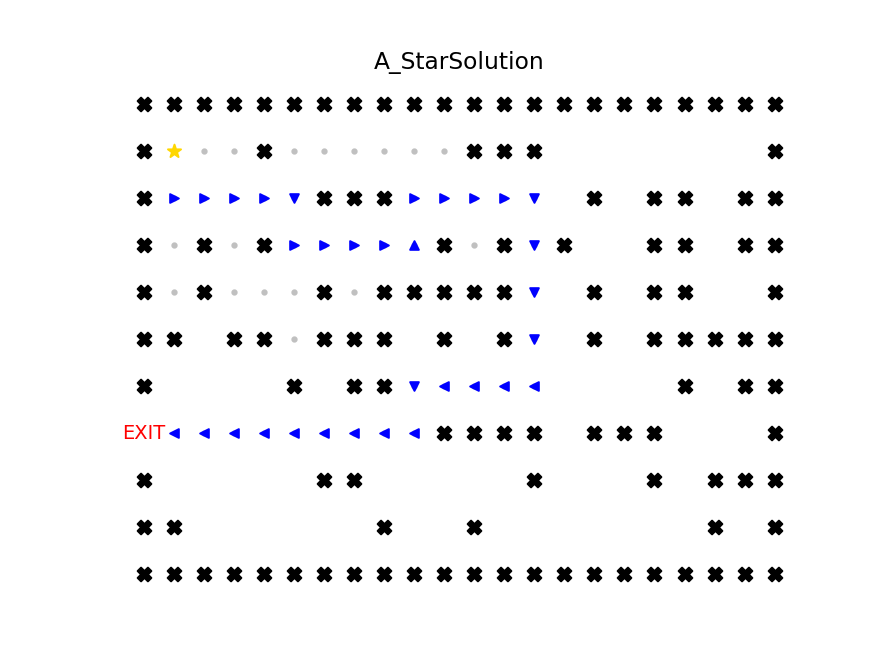
\includegraphics[width=8cm]{Figures/fg3_astar.png}
		\end{tabular}
	\end{figure}
	\begin{itemize}
		\item \textbf{Nhận xét}: Ta dễ dàng nhận thấy thuật toán DFS cho kết quả đường đi dài nhất và không tối ưu. Trong bản đồ này, thuật toán BFS lộ rõ nhược điểm của bản thân khi phải duyệt gần như toàn bộ các ô trong ma trận (kể cả những ô nửa bên phải vốn dĩ không cần duyệt qua). Thuật toán Greedy Best First Search do chịu ảnh hưởng của hàm heuristic (đã giải thích ở bản đồ 2) nên cho kết qủa dài dài hơn BFS và $A^{\star}$. Thuật toán  $A^{\star}$ cho kết quả tối ưu nhất nhưng lại tốn ít chi phí xử lí và bộ nhớ nhất.
	\end{itemize}
	

	
	\newpage
	\item Bản đồ 4:
	\begin{figure}[h] \label{bd4}
		\centering
		\begin{tabular}{cc}
			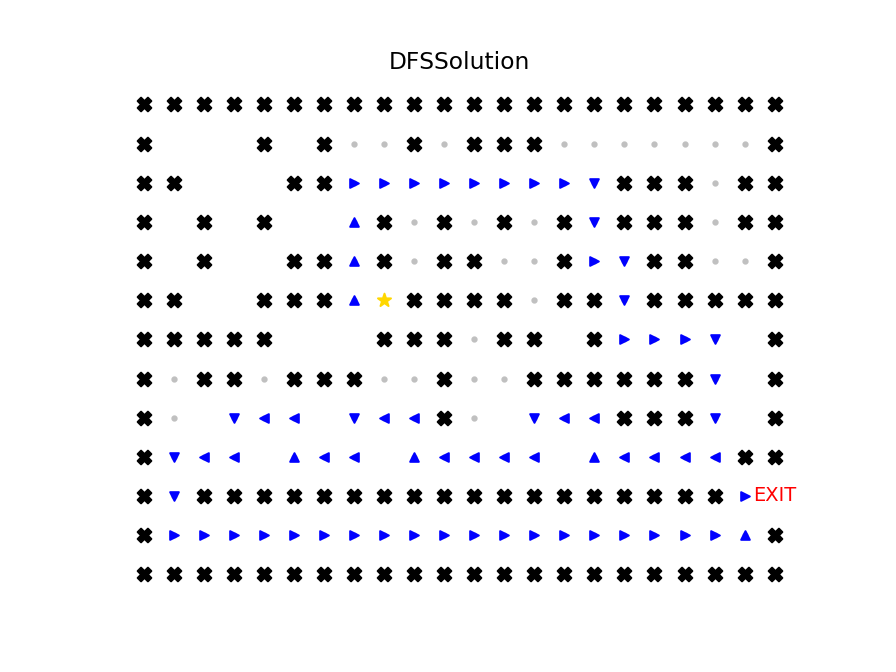
\includegraphics[width=8cm]{Figures/fg4_dfs.png} &
			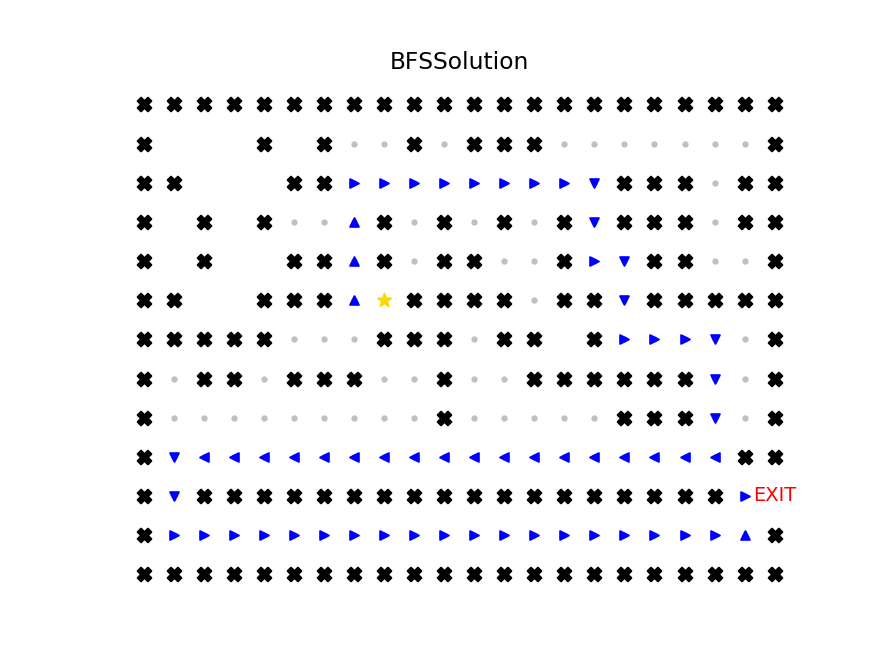
\includegraphics[width=8cm]{Figures/fg4_bfs.png} \\
		\end{tabular}
	\end{figure}
	\begin{figure}[h] \label{Hình 4}
		\centering
		\begin{tabular}{cc}
			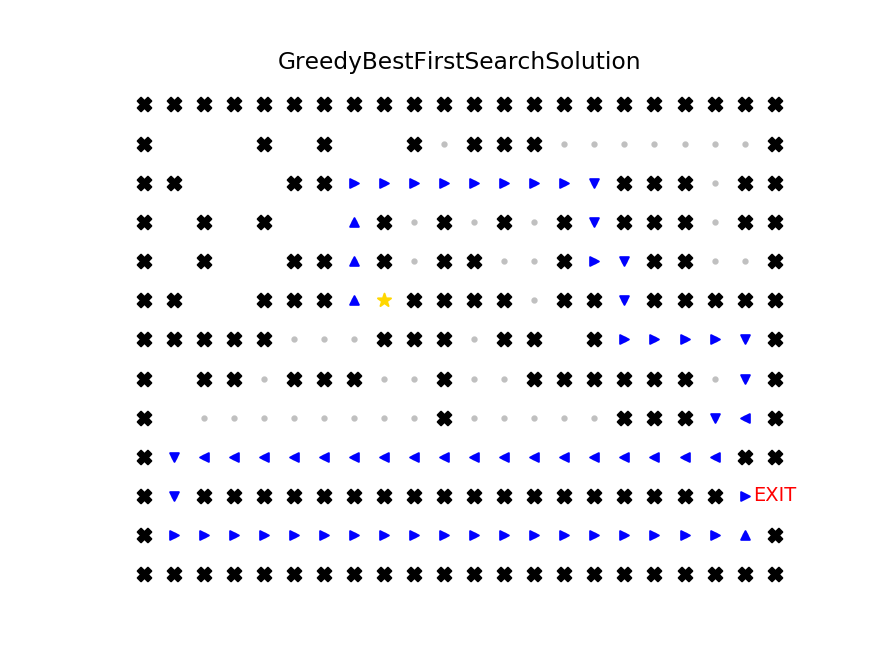
\includegraphics[width=8cm]{Figures/fg4_gbfs.png} &
			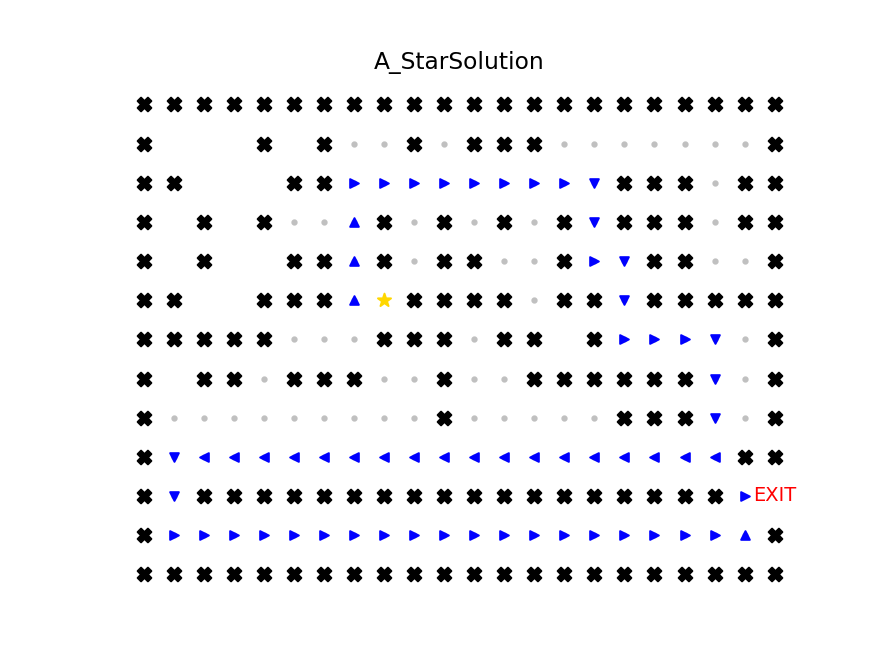
\includegraphics[width=8cm]{Figures/fg4_astar.png}
		\end{tabular}
	\end{figure}
	\begin{itemize}
		\item \textbf{Nhận xét}: Thuật toán DFS do duyệt theo chiều sâu và theo một nhánh duy nhất. Nhược điểm của thuật toán này lộ rõ khi bản đồ xuất hiện đoạn đường thẳng, thay vì đi thẳng tới đích thì thuật toán tạo ra đường đi hình ziczac do duyệt theo một nhánh duy nhất. Các thuật toán BFS, Greedy Best First Search và $A^{\star}$ cho kết quả khá tương đồng với nhau, và chênh lệch chi phí duyệt cũng không đáng kể.
	\end{itemize}

		\newpage
	\item Bản đồ 5:
	\begin{figure}[h] \label{bd5}
		\centering
		\begin{tabular}{cc}
			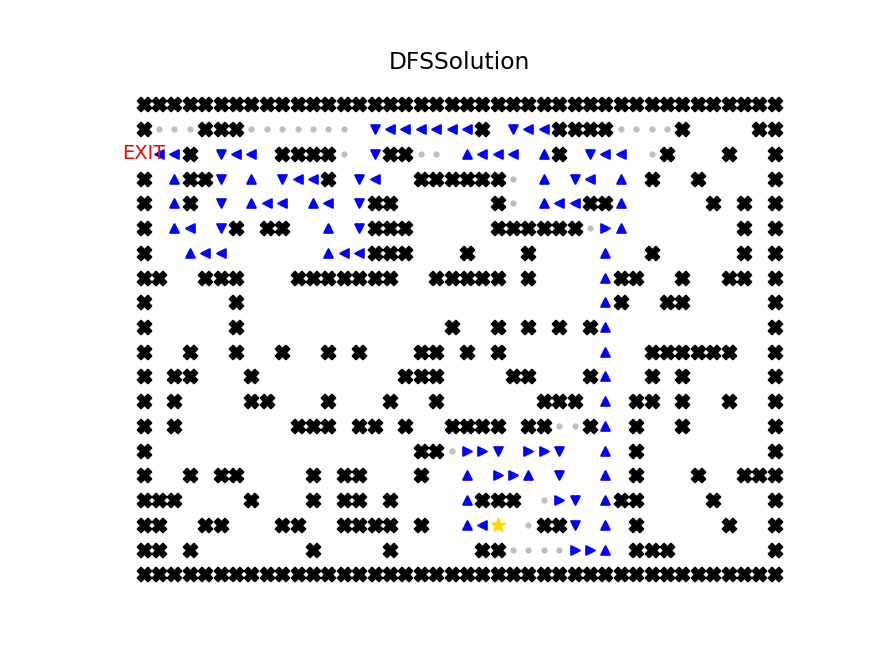
\includegraphics[width=8.5cm]{Figures/fg5_dfs.png} &
			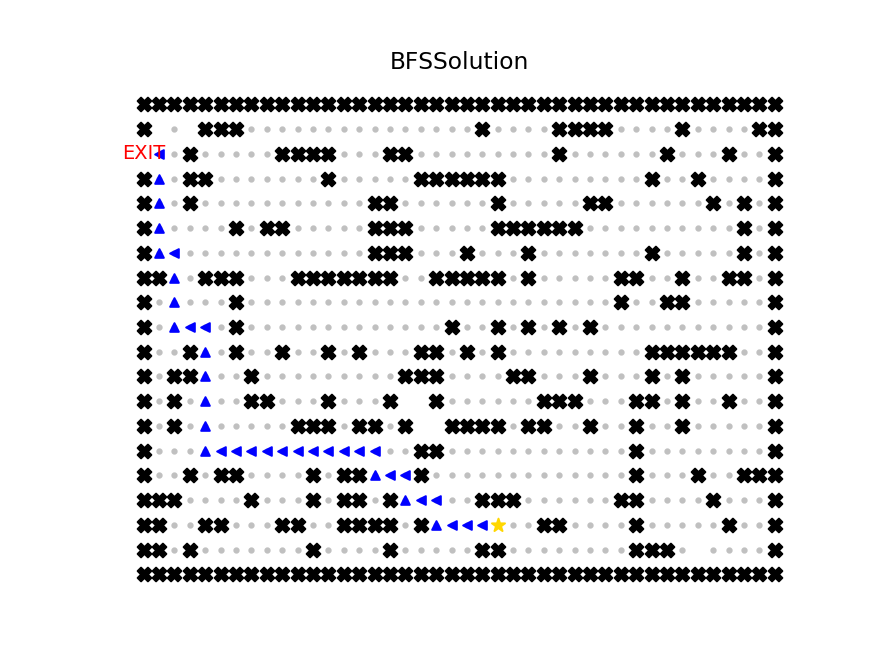
\includegraphics[width=8.5cm]{Figures/fg5_bfs.png} \\
		\end{tabular}
	\end{figure}
	\begin{figure}[h] \label{Hình 5}
		\centering
		\begin{tabular}{cc}
			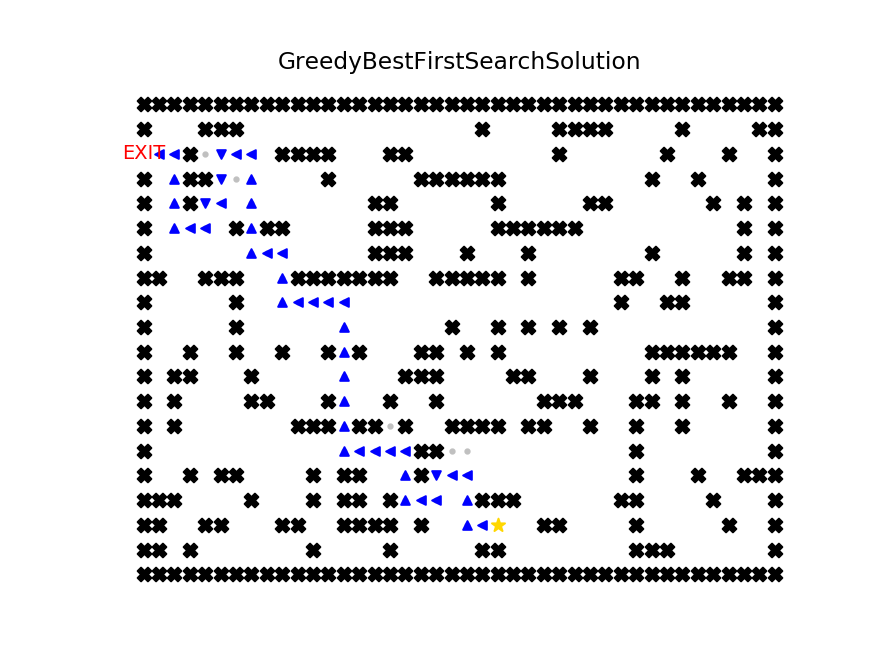
\includegraphics[width=8.5cm]{Figures/fg5_gbfs.png} &
			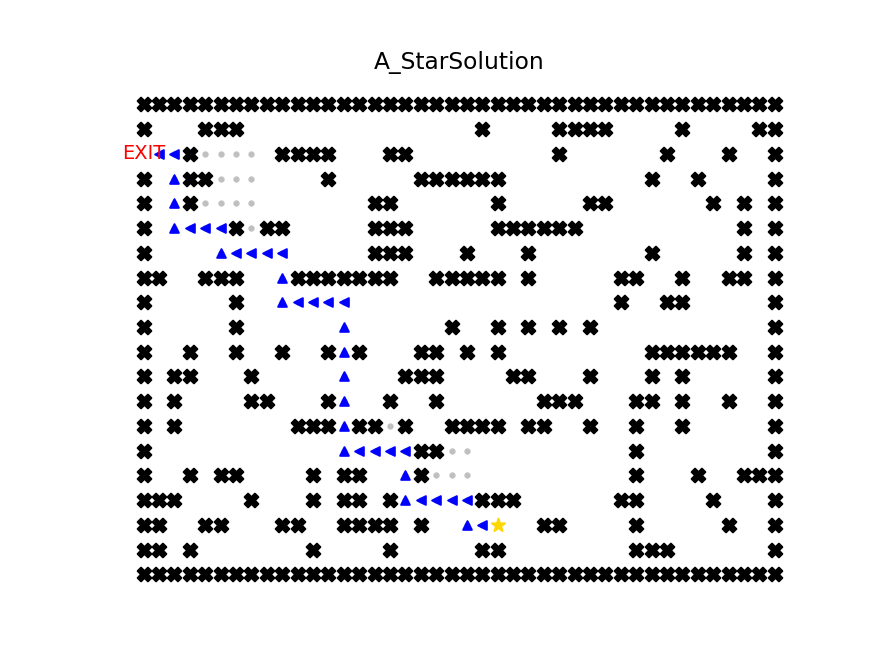
\includegraphics[width=8.5cm]{Figures/fg5_astar.png}
		\end{tabular}
	\end{figure}
	\begin{itemize}
		\item \textbf{Nhận xét}: Trong một bản đồ có kích thước lớn, thuật toán DFS vẫn cho ra kết quả đường đi dài nhất nhưng chi phí duyệt qua các ô tương đối ít. Trong khi đó, thuật toán BFS phải duyệt hầu hết các ô trong bản đồ mới tìm ra được đường đi ngắn nhất và tối ưu nhất. Thuật toán GreedyBestFirstSearch lại tiếp tục bị đánh lừa bởi những điểm gần lối thoát nhưng lại bị cản bởi vật cản, nên cho ra kết quả đường đi dài hơn BFS và $A^{\star}$. Mặc dù thuật toán BFS và $A^{\star}$ cho ra kết quả hai đường đi khác nhau nhưng chi phí đường đi thì tương đồng với nhau.
	\end{itemize}
	\end{itemize}

\newpage
\section{Bản đồ có điểm thưởng}
Ta biểu diễn cấu trúc bài toán điểm thưởng dưới dạng 1 bài toán tìm kiếm như sau:\\
- \textbf{Cấu trúc trạng thái}: là một list các điểm(bao gồm điểm thưởng, điểm bắt đầu, điểm đích) đã đi qua, điểm đi qua cuối cùng ở cuối list. \\
- \textbf{Trạng thái ban đầu} : là  list chỉ chứa điểm bắt đầu\\
- \textbf{Trạng thái kết thúc} : là list chứa điểm kết thúc\\
- \textbf{Hàm sinh trạng thái - Chi phí - Chuỗi hành động} :các trạng thái mới được sinh ra là các list mới được tạo ra bằng cách thêm \textbf{các điểm chưa đi qua} vào list cha. \textbf{Chi phí - Hành động} của trạng thái mới là \textbf{chi phí và dãy hành động} để di chuyển giữa \textbf{vị trí hiện tại} và \textbf{vị trí được thêm vào list}. Chi phí và dãy hành động giữa 2 điểm ấy có được nhờ vào việc thực hiện thuật toán \textbf{A*} (được cho là thuật toán tốt nhất để tìm đường đi giữa 2 điểm).\\
\emph{Có thể sẽ có thắc mắc nếu chi phí đi từ điểm thưởng này đến điểm thưởng kia là chi phí đi giữa 2 điểm thưởng \textbf{trên bản đồ}, vậy còn điểm thưởng được cộng vào ở đâu? Câu trả lời là trong lúc cài đặt bản đồ, nếu ô được đi tới có điểm thưởng thì chi phí thay vì là 1 sẽ là 1+ điểm thưởng.Việc cài đặt như vậy sẽ khiến bài toán tính đến trường hợp tồn tại điểm thưởng $C$ \textbf{trên đường đi} từ điểm thưởng $A$ đến điểm thưởng $B$}\\
Sau khi xây dựng xong trạng thái cho bài toán tìm kiếm với điểm thưởng. Ta chỉ cần sử dụng lại những giải thuật ở trên để giải bài toán ấy. Vì hàm heuristic cho bài toán được xây dựng ở trên \textbf{khá phức tạp} (chưa nghĩ ra), ta sẽ sử dụng thuật giải \textbf{UniformCostSearch} để tìm ra lời giải tối ưu nhất.\\
\subsection{Đánh giá thực nghiệm}
\begin{itemize}
	\item \textbf{Bản đồ 1}:
	\begin{figure}[h] % [h] forces the figure to be output where it is defined in the code (it suppresses floating)
		\centering
		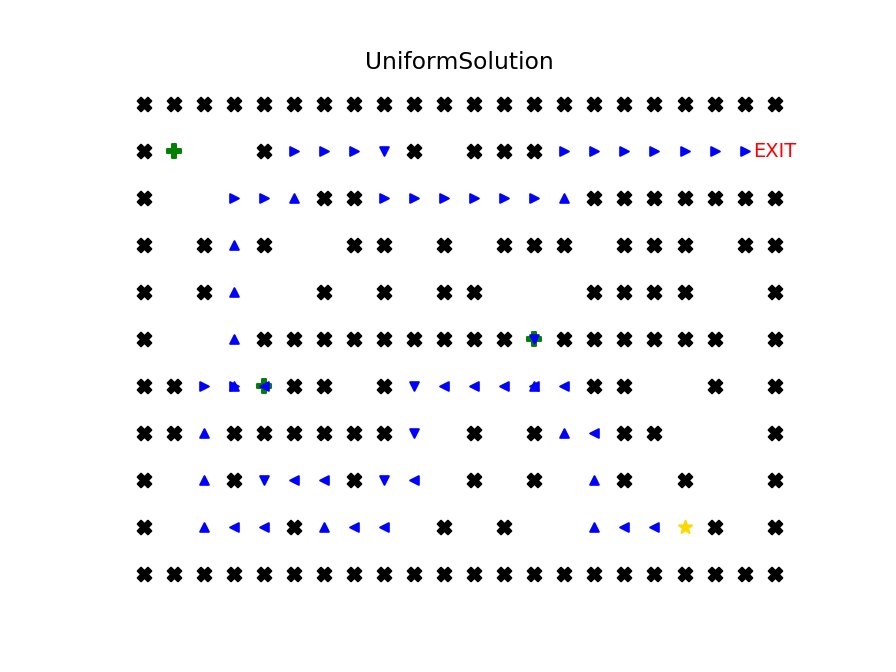
\includegraphics[width=0.8\columnwidth]{fg6.png} % Example image
	\end{figure}
	\begin{itemize}
		\item \textbf{Nhận xét}: Trong bản đồ này, ta có một điểm thưởng nằm ở góc trái của bản đồ không được chọn để đi qua. Bởi vì điểm thưởng này chỉ có giá trị là -4 mà chi phí để đi qua điểm thưởng này khá lớn nên sẽ không đi qua. Các điểm thưởng còn lại có chi phí đi tới để nhận khá thấp nên đều được đi qua và được nhận những điểm thưởng đó.
	\end{itemize}

	\newpage
	\item \textbf{Bản đồ 2}:
	\begin{figure}[h]
		\centering
		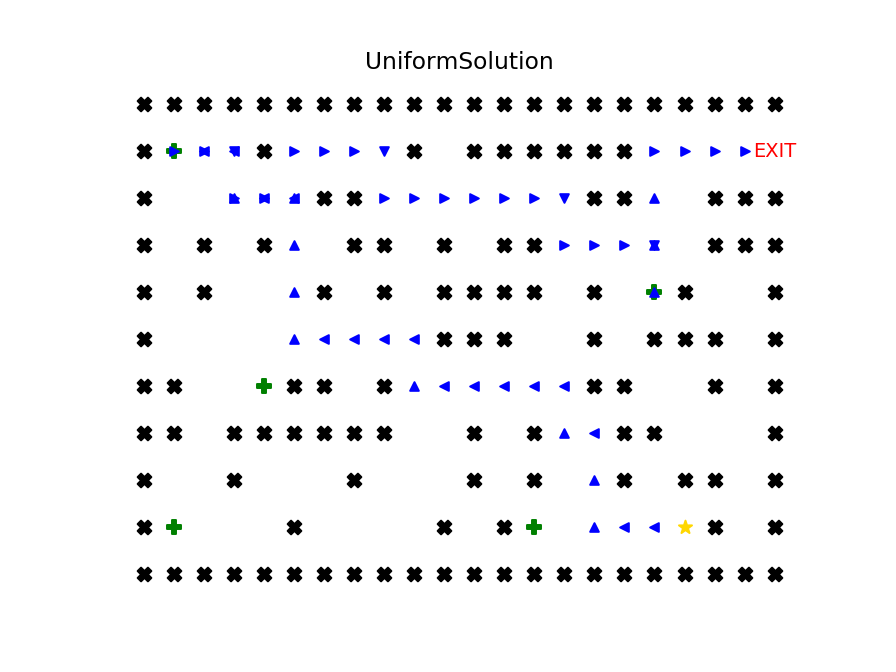
\includegraphics[width=0.8\columnwidth]{fg7.png} % Example image
	\end{figure}
	\begin{itemize}
		\item \textbf{Nhận xét}: Bản đồ này có một điểm thưởng ở góc trái. Dù chi phí để đi qua điểm thưởng đó khá lớn so với không đi qua điểm thưởng đó, nhưng giá trị điểm thưởng được cài đặt rất lớn (-50) nên vẫn sẽ đi qua điểm thưởng đó vì giá trị điểm thưởng mang lại cao hơn chi phí bỏ ra để đi qua điểm thưởng đó. 
	\end{itemize}

	\newpage
	\item \textbf{Bản đồ 3}:
	\begin{figure}[h]
		\centering
		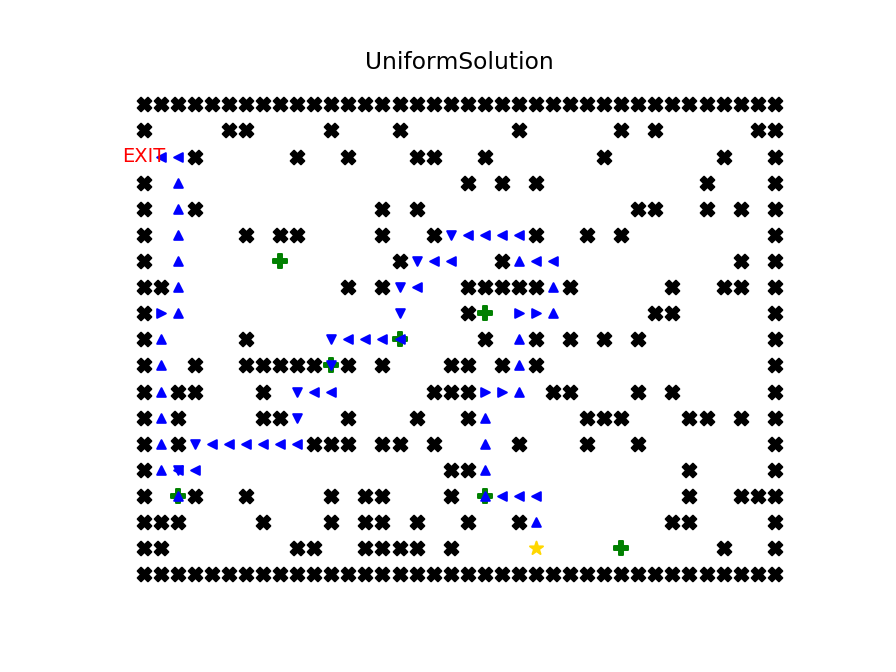
\includegraphics[width=0.8\columnwidth]{fg8.png} % Example image
	\end{figure}
	\begin{itemize}
		\item \textbf{Nhận xét}: Bản đồ này có một điểm thưởng dù nằm rất gần trên đường đi nhưng vẫn không được đi qua bởi vì giá trị của điểm thưởng đó khá thấp (chỉ là -1) nên xét về tính tối ưu thì sẽ không đi qua điểm thưởng đó. Ngược lại có một điểm thưởng ở góc dưới bên phải có giá trị -500 rất lớn nên sẽ được ưu tiên đi qua, đồng thời khi lựa chọn đường đi ấy, ta sẽ nhận được thêm một số điểm thưởng nằm bên cạnh đường đi ấy, từ đó sẽ tạo nên sự tối ưu khi vừa tìm được đường đi ngắn mà vẫn kiếm được nhiều điểm thưởng nhất.
	\end{itemize}
\end{itemize}

\bibliographystyle{plain}
\bibliography{ref}
\end{document}
